\documentclass[twoside]{book}

% Packages required by doxygen
\usepackage{fixltx2e}
\usepackage{calc}
\usepackage{doxygen}
\usepackage[export]{adjustbox} % also loads graphicx
\usepackage{graphicx}
\usepackage[utf8]{inputenc}
\usepackage{makeidx}
\usepackage{multicol}
\usepackage{multirow}
\PassOptionsToPackage{warn}{textcomp}
\usepackage{textcomp}
\usepackage[nointegrals]{wasysym}
\usepackage[table]{xcolor}

% Font selection
\usepackage[T1]{fontenc}
\usepackage[scaled=.90]{helvet}
\usepackage{courier}
\usepackage{amssymb}
\usepackage{sectsty}
\renewcommand{\familydefault}{\sfdefault}
\allsectionsfont{%
  \fontseries{bc}\selectfont%
  \color{darkgray}%
}
\renewcommand{\DoxyLabelFont}{%
  \fontseries{bc}\selectfont%
  \color{darkgray}%
}
\newcommand{\+}{\discretionary{\mbox{\scriptsize$\hookleftarrow$}}{}{}}

% Page & text layout
\usepackage{geometry}
\geometry{%
  a4paper,%
  top=2.5cm,%
  bottom=2.5cm,%
  left=2.5cm,%
  right=2.5cm%
}
\tolerance=750
\hfuzz=15pt
\hbadness=750
\setlength{\emergencystretch}{15pt}
\setlength{\parindent}{0cm}
\setlength{\parskip}{3ex plus 2ex minus 2ex}
\makeatletter
\renewcommand{\paragraph}{%
  \@startsection{paragraph}{4}{0ex}{-1.0ex}{1.0ex}{%
    \normalfont\normalsize\bfseries\SS@parafont%
  }%
}
\renewcommand{\subparagraph}{%
  \@startsection{subparagraph}{5}{0ex}{-1.0ex}{1.0ex}{%
    \normalfont\normalsize\bfseries\SS@subparafont%
  }%
}
\makeatother

% Headers & footers
\usepackage{fancyhdr}
\pagestyle{fancyplain}
\fancyhead[LE]{\fancyplain{}{\bfseries\thepage}}
\fancyhead[CE]{\fancyplain{}{}}
\fancyhead[RE]{\fancyplain{}{\bfseries\leftmark}}
\fancyhead[LO]{\fancyplain{}{\bfseries\rightmark}}
\fancyhead[CO]{\fancyplain{}{}}
\fancyhead[RO]{\fancyplain{}{\bfseries\thepage}}
\fancyfoot[LE]{\fancyplain{}{}}
\fancyfoot[CE]{\fancyplain{}{}}
\fancyfoot[RE]{\fancyplain{}{\bfseries\scriptsize Generated by Doxygen }}
\fancyfoot[LO]{\fancyplain{}{\bfseries\scriptsize Generated by Doxygen }}
\fancyfoot[CO]{\fancyplain{}{}}
\fancyfoot[RO]{\fancyplain{}{}}
\renewcommand{\footrulewidth}{0.4pt}
\renewcommand{\chaptermark}[1]{%
  \markboth{#1}{}%
}
\renewcommand{\sectionmark}[1]{%
  \markright{\thesection\ #1}%
}

% Indices & bibliography
\usepackage{natbib}
\usepackage[titles]{tocloft}
\setcounter{tocdepth}{3}
\setcounter{secnumdepth}{5}
\makeindex

% Hyperlinks (required, but should be loaded last)
\usepackage{ifpdf}
\ifpdf
  \usepackage[pdftex,pagebackref=true]{hyperref}
\else
  \usepackage[ps2pdf,pagebackref=true]{hyperref}
\fi
\hypersetup{%
  colorlinks=true,%
  linkcolor=blue,%
  citecolor=blue,%
  unicode%
}

% Custom commands
\newcommand{\clearemptydoublepage}{%
  \newpage{\pagestyle{empty}\cleardoublepage}%
}

\usepackage{caption}
\captionsetup{labelsep=space,justification=centering,font={bf},singlelinecheck=off,skip=4pt,position=top}

%===== C O N T E N T S =====

\begin{document}

% Titlepage & ToC
\hypersetup{pageanchor=false,
             bookmarksnumbered=true,
             pdfencoding=unicode
            }
\pagenumbering{roman}
\begin{titlepage}
\vspace*{7cm}
\begin{center}%
{\Large My Project }\\
\vspace*{1cm}
{\large Generated by Doxygen 1.8.11}\\
\end{center}
\end{titlepage}
\clearemptydoublepage
\tableofcontents
\clearemptydoublepage
\pagenumbering{arabic}
\hypersetup{pageanchor=true}

%--- Begin generated contents ---
\chapter{Class Index}
\section{Class List}
Here are the classes, structs, unions and interfaces with brief descriptions\+:\begin{DoxyCompactList}
\item\contentsline{section}{\hyperlink{structnode}{node} }{\pageref{structnode}}{}
\item\contentsline{section}{\hyperlink{structnode1}{node1} }{\pageref{structnode1}}{}
\item\contentsline{section}{\hyperlink{structnode__info}{node\+\_\+info} }{\pageref{structnode__info}}{}
\end{DoxyCompactList}

\chapter{File Index}
\section{File List}
Here is a list of all files with brief descriptions\+:\begin{DoxyCompactList}
\item\contentsline{section}{\hyperlink{Lab1_8c}{Lab1.\+c} }{\pageref{Lab1_8c}}{}
\end{DoxyCompactList}

\chapter{Class Documentation}
\hypertarget{classpath}{}\section{path Class Reference}
\label{classpath}\index{path@{path}}
\subsection*{Public Member Functions}
\begin{DoxyCompactItemize}
\item 
void \hyperlink{classpath_a1c4a54ae699c5583d464b0d904f2699a}{get} ()
\item 
void \hyperlink{classpath_af422edc0175627d75cfeb7dcad9b5ba3}{pm} ()
\item 
void \hyperlink{classpath_aa93bf33f14db6cd6312df7a66757060d}{ap} ()
\item 
void \hyperlink{classpath_a9eaa3e76753ed1540a877dd8a84aa5c3}{disp} ()
\end{DoxyCompactItemize}
\subsection*{Private Attributes}
\begin{DoxyCompactItemize}
\item 
int \hyperlink{classpath_a4c3e3313530b46fb13cd4b5163b03cb0}{n}
\item 
int \hyperlink{classpath_a74b571902c8e9e488f7bcc38630f0652}{p} \mbox{[}10\mbox{]}\mbox{[}10\mbox{]}
\item 
int \hyperlink{classpath_a73755051d4f15dd918791bc11b776521}{a} \mbox{[}10\mbox{]}\mbox{[}10\mbox{]}
\item 
int \hyperlink{classpath_a44e02858ba6e199f35611952bd5e42db}{c} \mbox{[}10\mbox{]}\mbox{[}10\mbox{]}
\end{DoxyCompactItemize}


\subsection{Member Function Documentation}
\index{path@{path}!ap@{ap}}
\index{ap@{ap}!path@{path}}
\subsubsection[{\texorpdfstring{ap()}{ap()}}]{\setlength{\rightskip}{0pt plus 5cm}void path\+::ap (
\begin{DoxyParamCaption}
{}
\end{DoxyParamCaption}
)}\hypertarget{classpath_aa93bf33f14db6cd6312df7a66757060d}{}\label{classpath_aa93bf33f14db6cd6312df7a66757060d}

\begin{DoxyCode}
82 \{
83     \textcolor{keywordtype}{int} i,j,k;
84     \textcolor{keywordflow}{for}(i=1;i<=\hyperlink{classpath_a4c3e3313530b46fb13cd4b5163b03cb0}{n};i++)
85     \{
86         \textcolor{keywordflow}{for}(j=1;j<=\hyperlink{classpath_a4c3e3313530b46fb13cd4b5163b03cb0}{n};j++)
87         \{
88 
89                 \hyperlink{classpath_a74b571902c8e9e488f7bcc38630f0652}{p}[i][j]=\hyperlink{classpath_a44e02858ba6e199f35611952bd5e42db}{c}[i][j];
90 
91         \}
92     \}
93     \textcolor{keywordflow}{for}(k=1;k<=\hyperlink{classpath_a4c3e3313530b46fb13cd4b5163b03cb0}{n};k++)
94     \{
95         \textcolor{keywordflow}{for}(i=1;i<=\hyperlink{classpath_a4c3e3313530b46fb13cd4b5163b03cb0}{n};i++)
96         \{
97             \textcolor{keywordflow}{for}(j=1;j<=\hyperlink{classpath_a4c3e3313530b46fb13cd4b5163b03cb0}{n};j++)
98             \{
99                 \textcolor{keywordflow}{if}(\hyperlink{classpath_a74b571902c8e9e488f7bcc38630f0652}{p}[i][j]<\hyperlink{classpath_a74b571902c8e9e488f7bcc38630f0652}{p}[i][k]+\hyperlink{classpath_a74b571902c8e9e488f7bcc38630f0652}{p}[k][j])
100                 \{
101                     \hyperlink{classpath_a74b571902c8e9e488f7bcc38630f0652}{p}[i][j]=\hyperlink{classpath_a74b571902c8e9e488f7bcc38630f0652}{p}[i][j];
102                 \}
103                 \textcolor{keywordflow}{else}
104                 \{
105                 \hyperlink{classpath_a74b571902c8e9e488f7bcc38630f0652}{p}[i][j]=\hyperlink{classpath_a74b571902c8e9e488f7bcc38630f0652}{p}[i][k]+\hyperlink{classpath_a74b571902c8e9e488f7bcc38630f0652}{p}[k][j];
106                 \}
107             \}
108         \}
109     \}
110     \hyperlink{classpath_af422edc0175627d75cfeb7dcad9b5ba3}{pm}();
111 \}
\end{DoxyCode}


Here is the call graph for this function\+:
\nopagebreak
\begin{figure}[H]
\begin{center}
\leavevmode
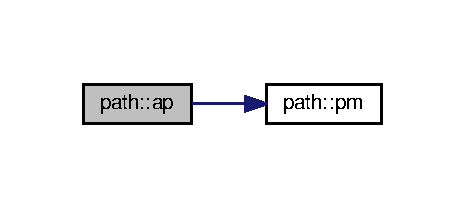
\includegraphics[width=223pt]{classpath_aa93bf33f14db6cd6312df7a66757060d_cgraph}
\end{center}
\end{figure}


\index{path@{path}!disp@{disp}}
\index{disp@{disp}!path@{path}}
\subsubsection[{\texorpdfstring{disp()}{disp()}}]{\setlength{\rightskip}{0pt plus 5cm}void path\+::disp (
\begin{DoxyParamCaption}
{}
\end{DoxyParamCaption}
)}\hypertarget{classpath_a9eaa3e76753ed1540a877dd8a84aa5c3}{}\label{classpath_a9eaa3e76753ed1540a877dd8a84aa5c3}

\begin{DoxyCode}
53 \{
54     cout<<\textcolor{stringliteral}{"The output matrix for the given graph is :"};
55     \textcolor{keywordflow}{for}(\textcolor{keywordtype}{int} i=1;i<=\hyperlink{classpath_a4c3e3313530b46fb13cd4b5163b03cb0}{n};i++)
56     \{
57         \textcolor{keywordflow}{for}(\textcolor{keywordtype}{int} j=1;j<=\hyperlink{classpath_a4c3e3313530b46fb13cd4b5163b03cb0}{n};j++)
58         \{
59             cout<<\hyperlink{classpath_a74b571902c8e9e488f7bcc38630f0652}{p}[i][j]<< \textcolor{stringliteral}{"  "};
60         \}
61         cout<<endl;
62 \}
63 \}
\end{DoxyCode}
\index{path@{path}!get@{get}}
\index{get@{get}!path@{path}}
\subsubsection[{\texorpdfstring{get()}{get()}}]{\setlength{\rightskip}{0pt plus 5cm}void path\+::get (
\begin{DoxyParamCaption}
{}
\end{DoxyParamCaption}
)}\hypertarget{classpath_a1c4a54ae699c5583d464b0d904f2699a}{}\label{classpath_a1c4a54ae699c5583d464b0d904f2699a}

\begin{DoxyCode}
18 \{
19     \textcolor{keywordtype}{int} i,j,k;
20     \textcolor{comment}{//clrscr();}
21     cout<<\textcolor{stringliteral}{"Enter the no. of nodes in the graph :"};
22     cin>>\hyperlink{classpath_a4c3e3313530b46fb13cd4b5163b03cb0}{n};
23     cout<<\textcolor{stringliteral}{"Enter the adjacency matrix :"};
24     \textcolor{keywordflow}{for}(i=1;i<=\hyperlink{classpath_a4c3e3313530b46fb13cd4b5163b03cb0}{n};i++)
25     \{
26         \textcolor{keywordflow}{for}(j=1;j<=\hyperlink{classpath_a4c3e3313530b46fb13cd4b5163b03cb0}{n};j++)
27         \{
28             \textcolor{comment}{//  cout<<"a["<<i<<","<<j<<"] = ";}
29             cin>>\hyperlink{classpath_a73755051d4f15dd918791bc11b776521}{a}[i][j];
30             \hyperlink{classpath_a74b571902c8e9e488f7bcc38630f0652}{p}[i][j]=0;
31         \}
32     \}
33     cout<<\textcolor{stringliteral}{"Enter The cost matrix is :"};
34     \textcolor{keywordflow}{for}(i=1;i<=\hyperlink{classpath_a4c3e3313530b46fb13cd4b5163b03cb0}{n};i++)
35     \{
36         \textcolor{keywordflow}{for}(j=1;j<=\hyperlink{classpath_a4c3e3313530b46fb13cd4b5163b03cb0}{n};j++)
37         \{
38            \textcolor{comment}{//   cout<<"a["<<i<<","<<j<<"] = ";}
39             cin>>\hyperlink{classpath_a44e02858ba6e199f35611952bd5e42db}{c}[i][j];
40         \}
41     \}
42     \textcolor{keywordflow}{for}(i=1;i<=\hyperlink{classpath_a4c3e3313530b46fb13cd4b5163b03cb0}{n};i++)
43     \{
44         \textcolor{keywordflow}{for}(j=1;j<=\hyperlink{classpath_a4c3e3313530b46fb13cd4b5163b03cb0}{n};j++)
45         \{
46 
47                 \hyperlink{classpath_a74b571902c8e9e488f7bcc38630f0652}{p}[i][j]=\hyperlink{classpath_a73755051d4f15dd918791bc11b776521}{a}[i][j];
48 
49         \}
50     \}
51 \}
\end{DoxyCode}
\index{path@{path}!pm@{pm}}
\index{pm@{pm}!path@{path}}
\subsubsection[{\texorpdfstring{pm()}{pm()}}]{\setlength{\rightskip}{0pt plus 5cm}void path\+::pm (
\begin{DoxyParamCaption}
{}
\end{DoxyParamCaption}
)}\hypertarget{classpath_af422edc0175627d75cfeb7dcad9b5ba3}{}\label{classpath_af422edc0175627d75cfeb7dcad9b5ba3}

\begin{DoxyCode}
66 \{
67     \textcolor{keywordtype}{int} i,j,k;
68 
69     \textcolor{keywordflow}{for}(k=1;k<=\hyperlink{classpath_a4c3e3313530b46fb13cd4b5163b03cb0}{n};k++)
70     \{
71         \textcolor{keywordflow}{for}(i=1;i<=\hyperlink{classpath_a4c3e3313530b46fb13cd4b5163b03cb0}{n};i++)
72         \{
73             \textcolor{keywordflow}{for}(j=1;j<=\hyperlink{classpath_a4c3e3313530b46fb13cd4b5163b03cb0}{n};j++)
74             \{
75                 \hyperlink{classpath_a74b571902c8e9e488f7bcc38630f0652}{p}[i][j]=\hyperlink{classpath_a74b571902c8e9e488f7bcc38630f0652}{p}[i][j] || \hyperlink{classpath_a74b571902c8e9e488f7bcc38630f0652}{p}[i][k] && \hyperlink{classpath_a74b571902c8e9e488f7bcc38630f0652}{p}[k][j];
76             \}
77         \}
78     \}
79 
80 \}
\end{DoxyCode}


\subsection{Member Data Documentation}
\index{path@{path}!a@{a}}
\index{a@{a}!path@{path}}
\subsubsection[{\texorpdfstring{a}{a}}]{\setlength{\rightskip}{0pt plus 5cm}int path\+::a\mbox{[}10\mbox{]}\mbox{[}10\mbox{]}\hspace{0.3cm}{\ttfamily [private]}}\hypertarget{classpath_a73755051d4f15dd918791bc11b776521}{}\label{classpath_a73755051d4f15dd918791bc11b776521}
\index{path@{path}!c@{c}}
\index{c@{c}!path@{path}}
\subsubsection[{\texorpdfstring{c}{c}}]{\setlength{\rightskip}{0pt plus 5cm}int path\+::c\mbox{[}10\mbox{]}\mbox{[}10\mbox{]}\hspace{0.3cm}{\ttfamily [private]}}\hypertarget{classpath_a44e02858ba6e199f35611952bd5e42db}{}\label{classpath_a44e02858ba6e199f35611952bd5e42db}
\index{path@{path}!n@{n}}
\index{n@{n}!path@{path}}
\subsubsection[{\texorpdfstring{n}{n}}]{\setlength{\rightskip}{0pt plus 5cm}int path\+::n\hspace{0.3cm}{\ttfamily [private]}}\hypertarget{classpath_a4c3e3313530b46fb13cd4b5163b03cb0}{}\label{classpath_a4c3e3313530b46fb13cd4b5163b03cb0}
\index{path@{path}!p@{p}}
\index{p@{p}!path@{path}}
\subsubsection[{\texorpdfstring{p}{p}}]{\setlength{\rightskip}{0pt plus 5cm}int path\+::p\mbox{[}10\mbox{]}\mbox{[}10\mbox{]}\hspace{0.3cm}{\ttfamily [private]}}\hypertarget{classpath_a74b571902c8e9e488f7bcc38630f0652}{}\label{classpath_a74b571902c8e9e488f7bcc38630f0652}


The documentation for this class was generated from the following file\+:\begin{DoxyCompactItemize}
\item 
\hyperlink{FloydWarshall_8cpp}{Floyd\+Warshall.\+cpp}\end{DoxyCompactItemize}

\chapter{File Documentation}
\hypertarget{FloydWarshall_8cpp}{}\section{Floyd\+Warshall.\+cpp File Reference}
\label{FloydWarshall_8cpp}\index{Floyd\+Warshall.\+cpp@{Floyd\+Warshall.\+cpp}}
{\ttfamily \#include $<$iostream.\+h$>$}\\*
{\ttfamily \#include $<$stdio.\+h$>$}\\*
{\ttfamily \#include $<$stdlib.\+h$>$}\\*
Include dependency graph for Floyd\+Warshall.\+cpp\+:
\nopagebreak
\begin{figure}[H]
\begin{center}
\leavevmode
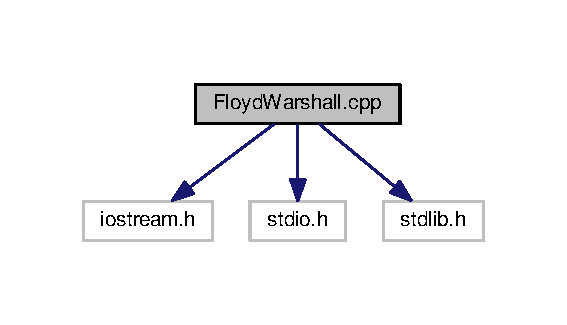
\includegraphics[width=272pt]{FloydWarshall_8cpp__incl}
\end{center}
\end{figure}
\subsection*{Classes}
\begin{DoxyCompactItemize}
\item 
class \hyperlink{classpath}{path}
\end{DoxyCompactItemize}
\subsection*{Functions}
\begin{DoxyCompactItemize}
\item 
void \hyperlink{FloydWarshall_8cpp_acdef7a1fd863a6d3770c1268cb06add3}{main} ()
\end{DoxyCompactItemize}


\subsection{Function Documentation}
\index{Floyd\+Warshall.\+cpp@{Floyd\+Warshall.\+cpp}!main@{main}}
\index{main@{main}!Floyd\+Warshall.\+cpp@{Floyd\+Warshall.\+cpp}}
\subsubsection[{\texorpdfstring{main()}{main()}}]{\setlength{\rightskip}{0pt plus 5cm}void main (
\begin{DoxyParamCaption}
{}
\end{DoxyParamCaption}
)}\hypertarget{FloydWarshall_8cpp_acdef7a1fd863a6d3770c1268cb06add3}{}\label{FloydWarshall_8cpp_acdef7a1fd863a6d3770c1268cb06add3}

\begin{DoxyCode}
113 \{
114 \hyperlink{classpath}{path} p;
115 p.\hyperlink{classpath_a1c4a54ae699c5583d464b0d904f2699a}{get}();
116 p.\hyperlink{classpath_af422edc0175627d75cfeb7dcad9b5ba3}{pm}();
117 cout<<\textcolor{stringliteral}{"path matrix is :"};
118 p.\hyperlink{classpath_a9eaa3e76753ed1540a877dd8a84aa5c3}{disp}();
119 \textcolor{comment}{//getch();}
120 p.\hyperlink{classpath_aa93bf33f14db6cd6312df7a66757060d}{ap}();
121 cout<<\textcolor{stringliteral}{"all pair shortest  path matrix is :"};
122 p.\hyperlink{classpath_a9eaa3e76753ed1540a877dd8a84aa5c3}{disp}();
123 \textcolor{comment}{//getch();}
124 \}
\end{DoxyCode}


Here is the call graph for this function\+:
\nopagebreak
\begin{figure}[H]
\begin{center}
\leavevmode
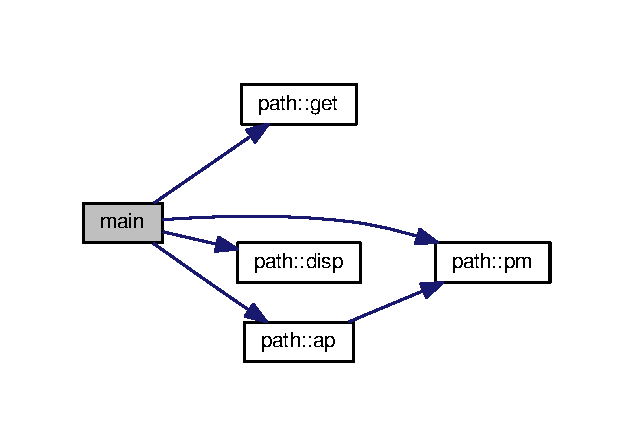
\includegraphics[width=304pt]{FloydWarshall_8cpp_acdef7a1fd863a6d3770c1268cb06add3_cgraph}
\end{center}
\end{figure}



%--- End generated contents ---

% Index
\backmatter
\newpage
\phantomsection
\clearemptydoublepage
\addcontentsline{toc}{chapter}{Index}
\printindex

\end{document}
